\section{Case Study}

\subsection{Scenario Generation}




\subsection{Results}
Considering different values for risk aversion, we wish to compare a hybrid producer's revenue with the sum of two single energy producers' revenues, i.e.\ the sum of the revenues of a solar only producer and a wind power only producer. The way we modelled the problem, it was possible to simply neglect one energy source by setting the respective parameters to zero. Consequently, we could use the sam emodel for all three producers. Apart from that, we optimised the revenue once for the situation with an adjustment market and once for the situation without an adjustment market. The results are summarised in the figures below.  

\begin{figure}[h!]
	\centering
	
	\begin{minipage}{0.95\textwidth}
		\subfloat[]{
			\centering
			\scalebox{0.75}{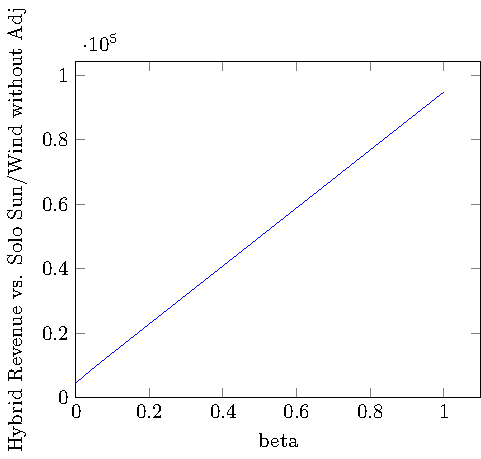
\includegraphics[]{Figures/figure2.pdf}}
		}
		\hfill
		\subfloat[]{
			\centering
			\scalebox{0.75}{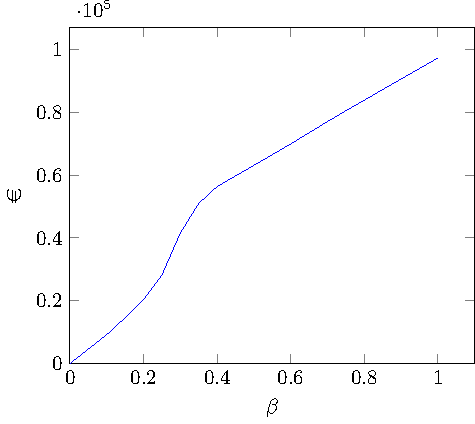
\includegraphics[]{Figures/figure.pdf}}
		}
		
		\caption{Revenue }\label{fig:overyear}
	\end{minipage}	
\end{figure}

We plotted the difference in the revenue of the hybrid producer and the sum of both single producers' revenues on the vertical axis. We presented the risk aversion factor $\beta$ on the horizontal axis. Overall, we see that the hybrid model is more advantageous for risk-averse producers. The more risk-averse a producer is, the more profitable it is to offer solar and wind power collectively. One striking difference is that the curve on the right starts in the origin while the curve on the left does not. If we have an adjustment market and are not risk-averse, it does not matter whether one producer offers both energies or two producers offer one energy each. The reason is that a risk-seeking producer offers everything on the day-ahead market and plans on buying back the deficit on the adjustment market. This is due to him expecting a lower price on the adjustment market than on the day-ahead market for our given data.
On the other hand, if we do not have an adjustment market, we can exploit the anti-correlation. Thus, the variance of the produced amount of energy decreases and therefore, the hybrid producer can offer more energy for a given day-ahead price. Hence, it is more profitable to produce both collectively. 

Apart from that, we observe a linear growth behaviour in a market system without an adjustment market. When adding the adjustment market to the system, we notice a slight bump. At some value for the risk aversion factor $\beta$, the producer is not brave enough anymore to trade on arbitrage since he would face losses in specific scenarios. 